\documentclass[a4paper,10pt]{report}
\usepackage[utf8]{inputenc}

% Title Page
\title{Architecture of E-Health Flanders platform}
\author{}


\begin{document}
\maketitle

\begin{abstract}
\end{abstract}

\part{Documentation Beyound Views}

\section{Documentation roadmap}

\subsection{Description of the parts}

\subsection{How stakeholders might use the package}

\subsubsection{Platform tester}

\subsubsection{Patient}

\subsubsection{Government}

\section{View template}

\section{System overview}

\section{Mapping between views}

\section{Directory}

\section{Glossary and acronym list}

\section{Background, design constraints, and rationale}



\part{Software Architecture Views}

\section{Module Uses View}

\subsection{Primary presentation}



\subsection{Element catalog}

\subsubsection{Elements and their properties}

\subsubsection{Relations and their properties}

\subsubsection{Element interfaces}

\subsubsection{Element behavior}

\subsection{Context diagram}

\subsection{Variability guide}

\subsection{Architecture background}

\subsubsection{Rationale}

\subsubsection{Analysis results}

\subsubsection{Assumptions}

\subsection{Other information}

\subsection{Related view packets}




\section{C\&C Client and Server View: Overview}

\subsection{Primary presentation}

\begin{center}
    \begin{figure}
      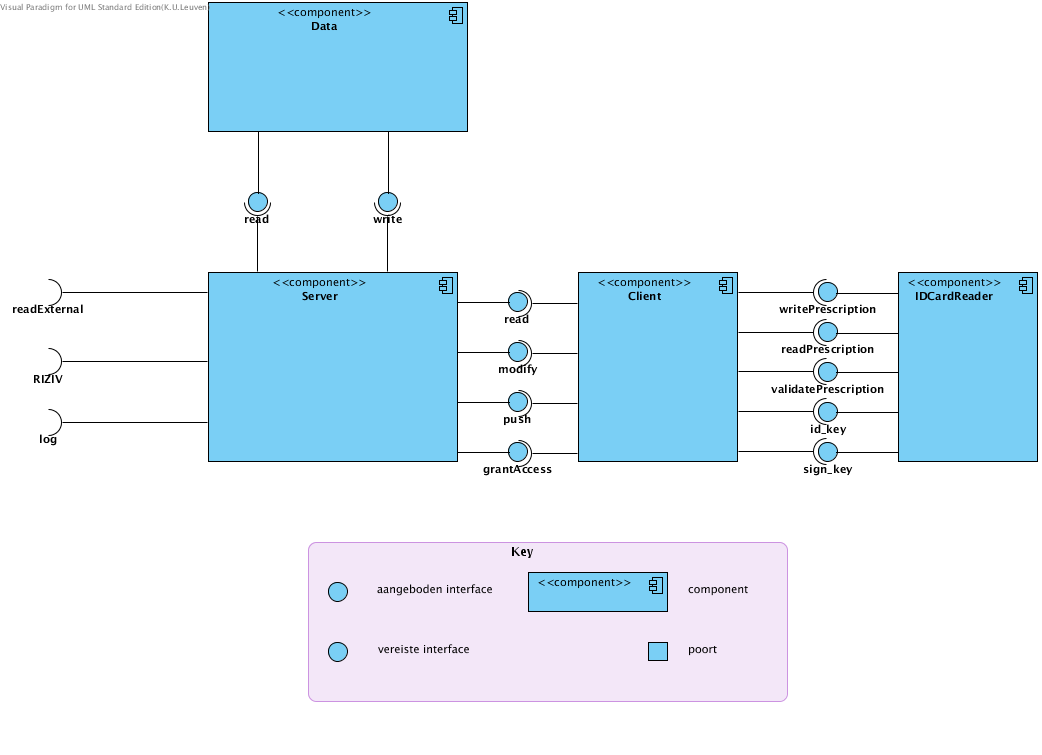
\includegraphics{../images/ClientServer_Overview.png}
    \end{figure}
  \end{center}
\end{frame}



\subsection{Element catalog}

\paragraph{Server}
The server is the component where clients can connect to, to interact in a save way.  The server is connected to clients, a government server, external components and the data server.  More information can be found in Client and Server view: Server.
%TODO location

\paragraph{Client}
The client component is the hub from where users (doctors, patients or pharmacists) can interact with the server in a save way.  More information can be found in Client and Server view: Client.
%TODO location

\paragraph{Data}
De data component is een database waar alle informatie zoals patienten dossiers en dokter data op bewaard zijn.  Hoe de data precies wordt opgeslaan is terug te vinden in het Deployment diagram.
%TODO location

\paragraph{Card}
De card component stelt de e-Card van de gebruiker voor.  De e-Card bevat gebruikersinformatie alsook twee keys.  Een key voor identificatie van de gebruiker en een key voor authenticatie.  Naast de gebruikersinformatie en de keys heeft de e-Card ook ruimte voor een aantal voorschriften op te slaan.  Meer informatie is terug te vinden in:
%TODO location

\paragraph{Government}
De government component bevat de logging en RIZIV database.

\paragraph{External}
De external component bevat de validated data sources die gebruikers van de client kunnen opvragen via de server.

%TODO government en external => context diagram?


\subsection{Context diagram}
TODO
%TODO

\subsection{Variability guide}
[None]

\subsection{Architecture background}
%TODO

\subsubsection{Rationale}
Enkele design beslissingen die hier te zien zijn is het gebruik van de card reader voor het identifici\"{e}ren van de gebruikers op de centrale database, meer hierover is te vinden in het ...TODO.
%TODO security
%TODO voorschriften.

\subsection{Related view packets}
De volgende client-server views bekijken dit overview diagram in meer detail.  Ook in het deployment diagram is extra informatie te vinden vooral dan in verband met de opslag van de global medical records en dokter data.



\section{Allocation Deployment View}

\subsection{Primary presentation}
Gewoon om te testen wat invloed van tekst is.

\subsection{Element catalog}

\subsubsection{Elements and their properties}

\subsubsection{Relations and their properties}

\subsubsection{Element interfaces}

\subsubsection{Element behavior}

\subsection{Context diagram}

\subsection{Variability guide}

\subsection{Architecture background}

\subsubsection{Rationale}

\subsubsection{Analysis results}

\subsubsection{Assumptions}

\subsection{Other information}

\subsection{Related view packets}



\section{Interaction Diagrams}

\subsection{Primary presentation}

\subsection{Element catalog}

\subsubsection{Elements and their properties}

\subsubsection{Relations and their properties}

\subsubsection{Element interfaces}

\subsubsection{Element behavior}

\subsection{Context diagram}

\subsection{Variability guide}

\subsection{Architecture background}

\subsubsection{Rationale}

\subsubsection{Analysis results}

\subsubsection{Assumptions}

\subsection{Other information}

\subsection{Related view packets}

\end{document}          
